\documentclass[A4]{article}
\usepackage{amsmath}
\usepackage{listingsutf8}
\lstset{literate={č}{{\v c}}1 {š}{{\v s}}1 {ž}{{\v z}}1} %Paket listings (oz. listingsutf8) direktno ne podpirata šumnikov.
\lstset{basicstyle=\ttfamily, language=Octave} %Nastavimo, da je privzet jezik za lstlistings octave.
\usepackage[pdftex]{graphicx}
\usepackage[english]{babel} % slovenske nastavitve (naslovi, deljenje besed ...)
\usepackage[T1]{fontenc}    % font encoding; T1 podpira slovenščino
\usepackage[utf8]{inputenc} % input encoding; lahko je tudi [cp1250] ali [latin2]
\usepackage{graphicx}
\usepackage{amsmath}
\usepackage{amssymb}
\usepackage{float}
\usepackage{subfig}
\usepackage{graphicx}
\usepackage[export]{adjustbox}

\newcommand{\R}{\mathbb{R}}

\begin{document}
\title{Lens Simulation}
\author{Jernej Vivod, Kim Ana Badovinac, Katja Logar}
\maketitle
\section{Description}

\section{Problem Statement}

In this group project we were tasked with implementing a simple ray tracing model capable of simulating ray refraction cause by an optical lens represented by an implicit function. We implemented the project using the MATLAB programming language and also provided a simple user interface for interacting with the simulation.

\section{Screens and Rays}

We started work on the project by implementing the two screens that were to provide the means to trace and visually represent the path of rays and how the change of the path changes the provided image. \\\\
Both screens were represented as a point in space corresponding to the upper left corner and two vectors spanning the parallelogram representing the screen. The rays were modelled as a parametrized line function. \\\\
The natural next step was to compute line equations each representing a ray going from a point representing a light source and through each pixel of the image on the first screen represented as a 2 dimensional matrix. This was achieved by dividing the parallelogram representing the screen into squares of equal size and getting the coordinates of the centres of each square. \\\\
This was achieved using the functions \textbf{\textit{get\_pixel\_coordinates}} and its auxiliary function \textbf{\textit{get\_coordinates}}. The function \textbf{\textit{get\_pixel\_coordinates}} returns a cell array containing at indices pair $(i, j)$ the coordinates of the pixel with indices $(i, j)$. The source code for these two functions can be found in the screens folder. \\\\
This matrix of line functions represents a sort of interface between the three main modules of the program. The first module generates, with respect to light source position and first screen position, size and shape, the cell array of line functions representing the rays as they leave each pixel of the first screen. This matrix serves as the input to the second module performing the actual lensing and, modified by the second module, is also the input to the third module that then actually computes the intersection coordinates and the indices of pixels that were intersected by the rays on the second screen.  

\vspace{10mm}

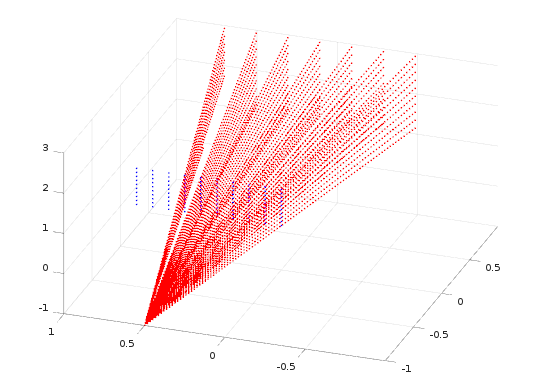
\includegraphics[scale=0.5, inner]{rays1}
\captionof{figure}{Visualizing the Rays Passing from the Light Source Through each Pixel on the Second Screen}

\vspace{10mm}

\section{Computing Intersections with the Second Screen}

This section describes the workings of the so called third module that takes the cell array of line functions representing the rays processed by the second module (which applies lensing). This is a well known problem of computing the intersection of a line with with a plane spanned by the two vectors representing the second screen. \\\\
A point on the plane can be represented as a linear combination given by
\[
P_{0} + P_{01}u + P_{02}v, \\ u, v \in R
\]
Where $P_{01}$ and $P_{02}$ are vectors from a point on the plane to the tips of the spanning vectors $u$ and $v$ respectively. \\\\
The point at which the line intersects the plane s therefore described by setting the point on the line equal o the point on the plane, giving the parametric equation
\[
l_{a} + l_{ab}t = P_{0} + P_{01}u + P_{02}v
\]
Where $l_{a}$ is a point on the line and $l_{ab}$ is the line's directional vector. \\\\
Rewritten, these equations can be expressed in matrix form as
\[
\begin{bmatrix} l_{a} - P_{0}\end{bmatrix} = \begin{bmatrix} -l_{ab} \ P_{01} \ P_{02}\end{bmatrix} \begin{bmatrix} t \\ u \\ v \end{bmatrix}
\]
This system of of linear equations can now be solved for $t, u$ and $v$. The point of intersection can then be computed by plugging the solution for $t$ back into the line equation. We can also check if the intersection actually happened on the screen, that is, the parallelogram spanned by the two vectors. This fact can be establishing by inspecting the results for the spanning vector scaling coefficients that we got by solving the system of linear equations. If they are elements of $[0, 1]$ the intersection happened on the parallelogram and hence the second screen. \\\\
For getting the actual indices of the pixels that were intersected the second screen can be divided in a similar fashion to what was done to the first screen when we computed the coordinates of each pixels. Performing a kind of inverse computation we can use similar reasoning to get the index pair $(i, j)$ from the coordinates of intersection. \\\\
This allows us to get a mapping from pixels on the second screen to the pixels on the first screen which consequently makes it possible to assign to the pixels on the first screen the color of the pixel that was intersected by the ray corresponding to this pixel on the second screen. \\

\section{Refraction}
When light passes through media with different indices of refraction, it refracts according to Snell's law. Snell's law tells us that the ratio of the sines of the angles of incidence and refraction is equivalent to the ratio of the indices of refraction:
\[
	\dfrac{\sin(\theta_1)}{\sin(\theta_2)} = \dfrac{n_2}{n_1}
\]
In the above equation, $\theta_1$ in the angle of incidence (the angle between the ray of incidence and the normal to the surface), $\theta_2$ in the angle of refraction (the angle between the ray of refraction and the normal to the surface), $n_1$ is the refractive index of the incoming medium and $n_2$ is the refractive index of the outcoming medium. \\ \\
In our project we notice refraction when the ray enters the len and when it exits the len. \\ \\
Refraction is implemented in function $refraction.m$. Instead of the scalar form of the law, we use Snell's law in vector form:
\[
	\vec{s_2} = \dfrac{n_1}{n_2}(\vec{n}\times(-\vec{n}\times\vec{s_1})) - \vec{n}\sqrt{1-(\dfrac{n_1}{n_2})^2(\vec{n}\times\vec{s_1})(\vec{n}\times		\vec{s_1})}
\]
Here $\vec{s_2}$ is the vector we seek, meaning it is the refracted vector, $\vec{s_1}$ is the incident vector and $\vec{n}$ is the normal, that we compute by computing the gradient of the function of the len at the intersection. \\ \\
It is important to note, that the above formula assumes, that both $\vec{n}$ and $\vec{s_1}$ are vectors with the norm equal to 1. Therefore, before we compute $\vec{s_2}$, we need to divide $\vec{n}$ and $\vec{s_1}$ by their norm. \\\\
Also, when computing the refracted ray, it is important to know, whether we are entering the len or exiting it. That is because the first part of the above equation: $\dfrac{n_1}{n_2}(\vec{n}\times(-\vec{n}\times\vec{s_1}))$ contains $-$ in $(-\vec{n}\times\vec{s_1})$, which takes into consideration that we should actually take the negative normal, when entering the len, since the negative normal points in the same direction (towards the center) as the incident ray. Therefore, the $-$ in  $(-\vec{n}\times\vec{s_1})$ is not needed when we are exiting the len.\\ \\
One more thing that we have to watch out for is total internal reflection. It can happen for rays that are crossing into a less dense medium ($n_2 < n_1$) - in our case that happens when light exits the len. In that case, if the incident angle is big enough, the light won't refract, it will reflect. That happens for angles bigger than the critical angle. \\\\

\subsubsection{Alternative method for computing the refracted ray}
We can compute the orthogonal projection of the incident vector to the normal of the surface:
\[
	\vec{p} = \dfrac{\vec{s_1} \vec{n}}{\vec{n} \vec{n}}\vec{n}
\]
Then we compute the vector $\vec{u}$:
\[
	\vec{u} = \vec{s_1} - \vec{p}
\]
The refracted ray is then:
\[
	\vec{s_2} = \vec{p} + \dfrac{n_1}{n_2}\vec{u}
\]

\vspace{10mm}

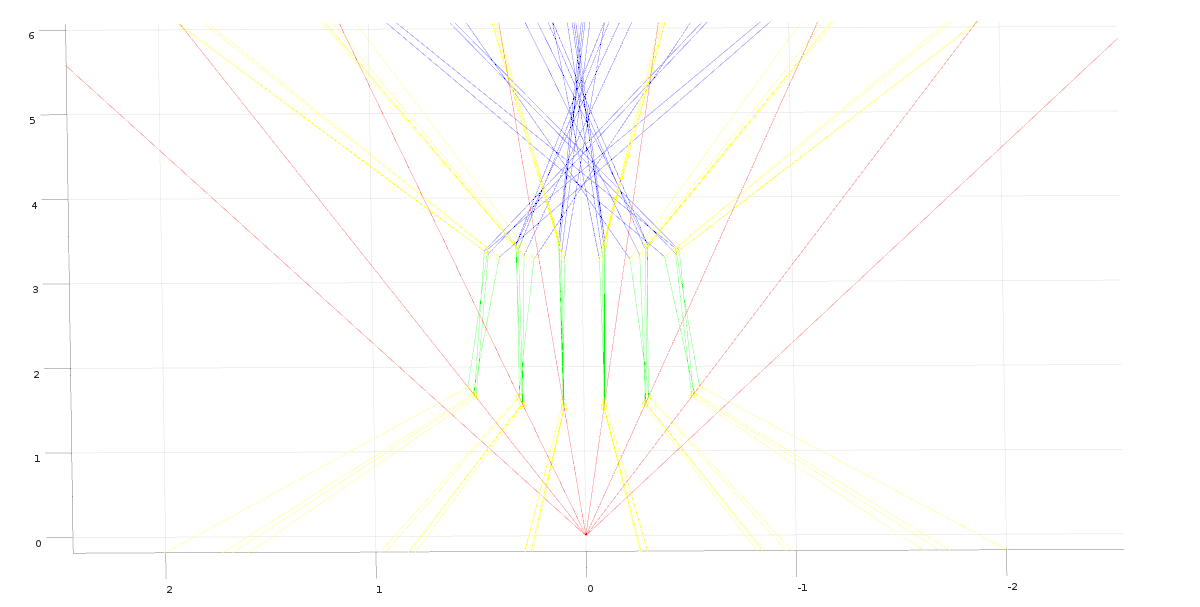
\includegraphics[scale=0.3]{rays_in}
\captionof{figure}{Visualizing the Rays entering a Spherical lens}

\vspace{10mm}

\section{Results}

This section presents some images that were obtained by running the program. The program is configured to be able to produce both images with applied lensing and also plots of the light source, screens and lens configuration that produced these results.\\\\
An extended collection of the results can be found in the results folder in the the project folder.


\vspace{10mm}


\includegraphics[scale=0.3]{cat}
\captionof{figure}{The Original image of a Cat used for Testing Purposes}

\vspace{10mm}


\includegraphics[scale=0.5]{checkers}
\captionof{figure}{The Original Image of A Checkers Pattern used for Testing Purposes}

\vspace{10mm}

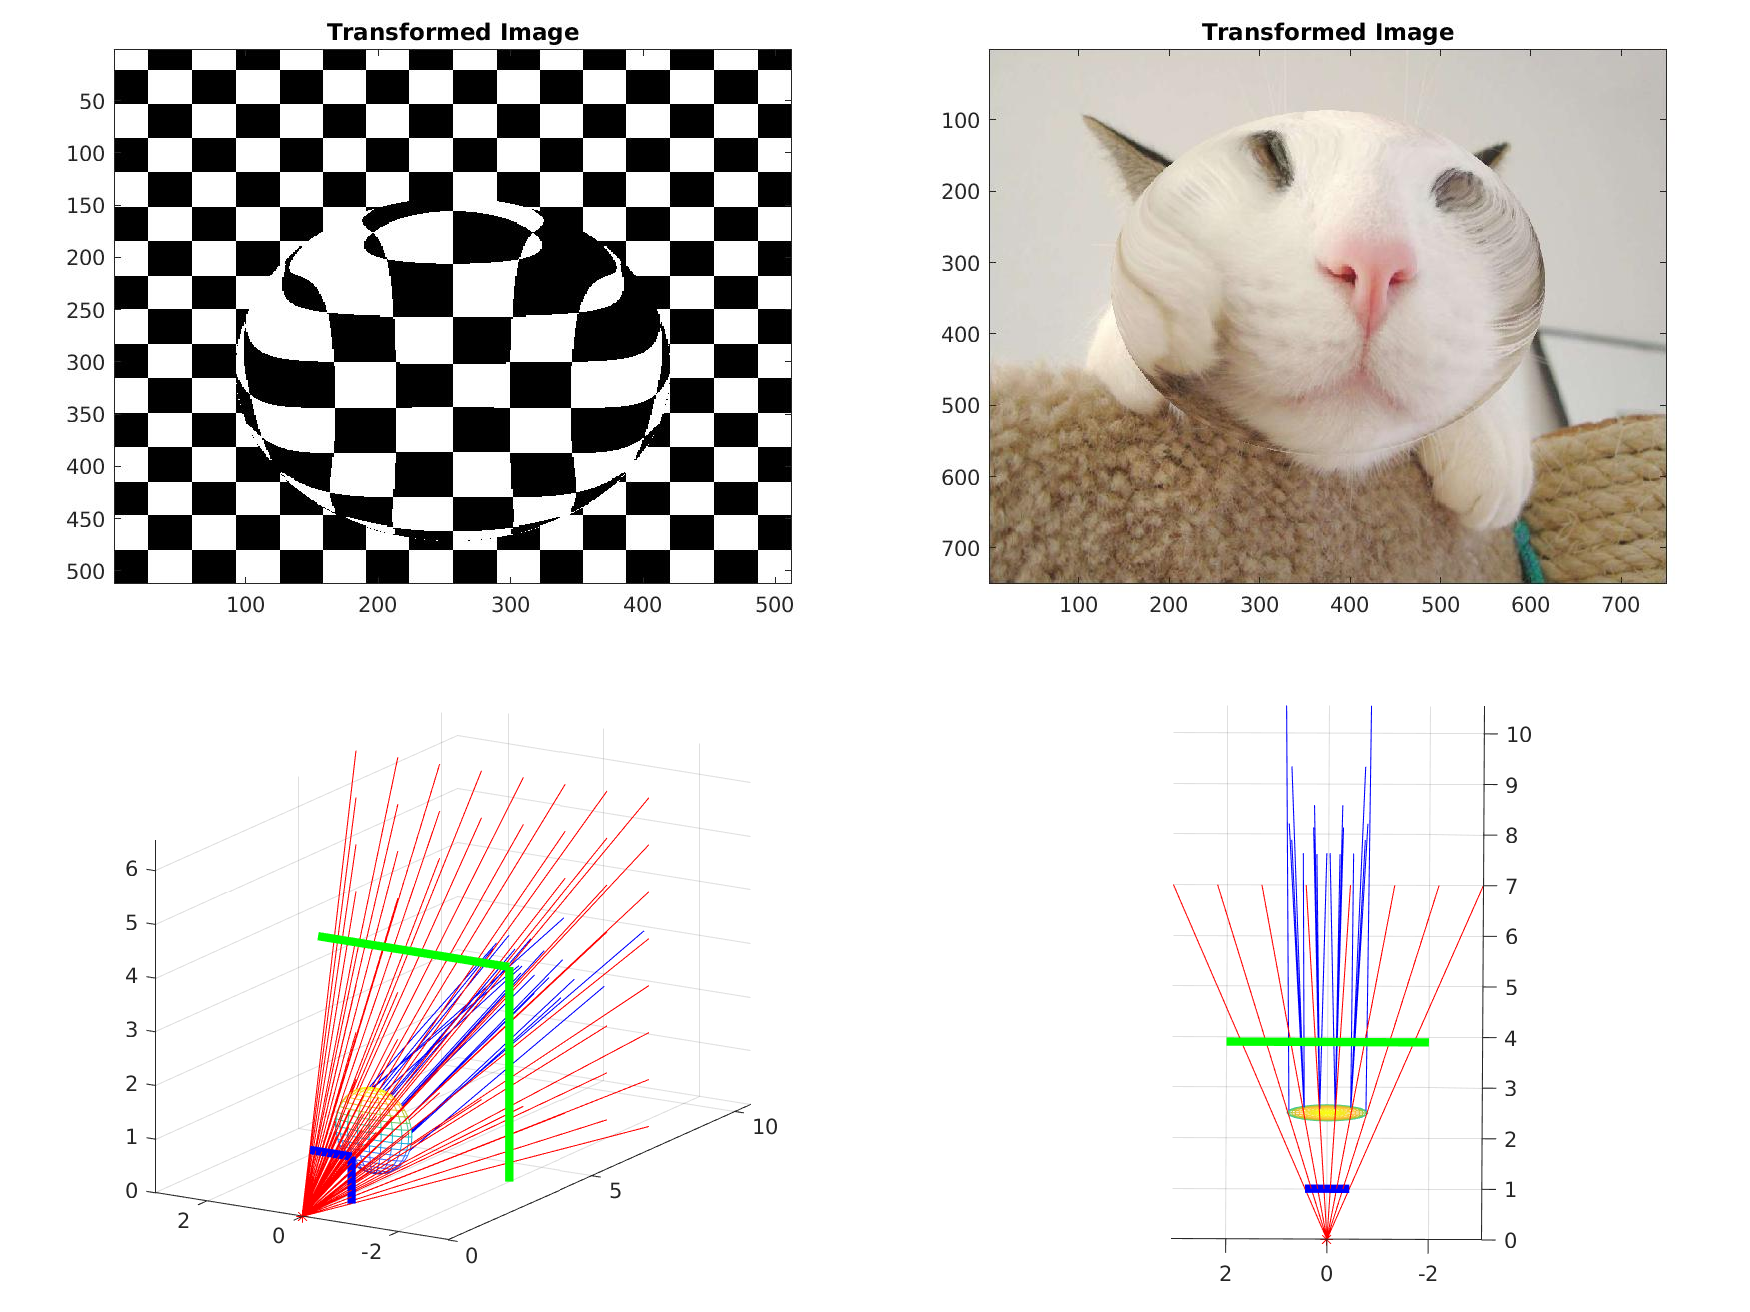
\includegraphics[scale=0.18, inner]{1}
\captionof{figure}{Applying an Ellipsoidal lens with an 0.2 Scaling factor in the x Direction}

\vspace{10mm}

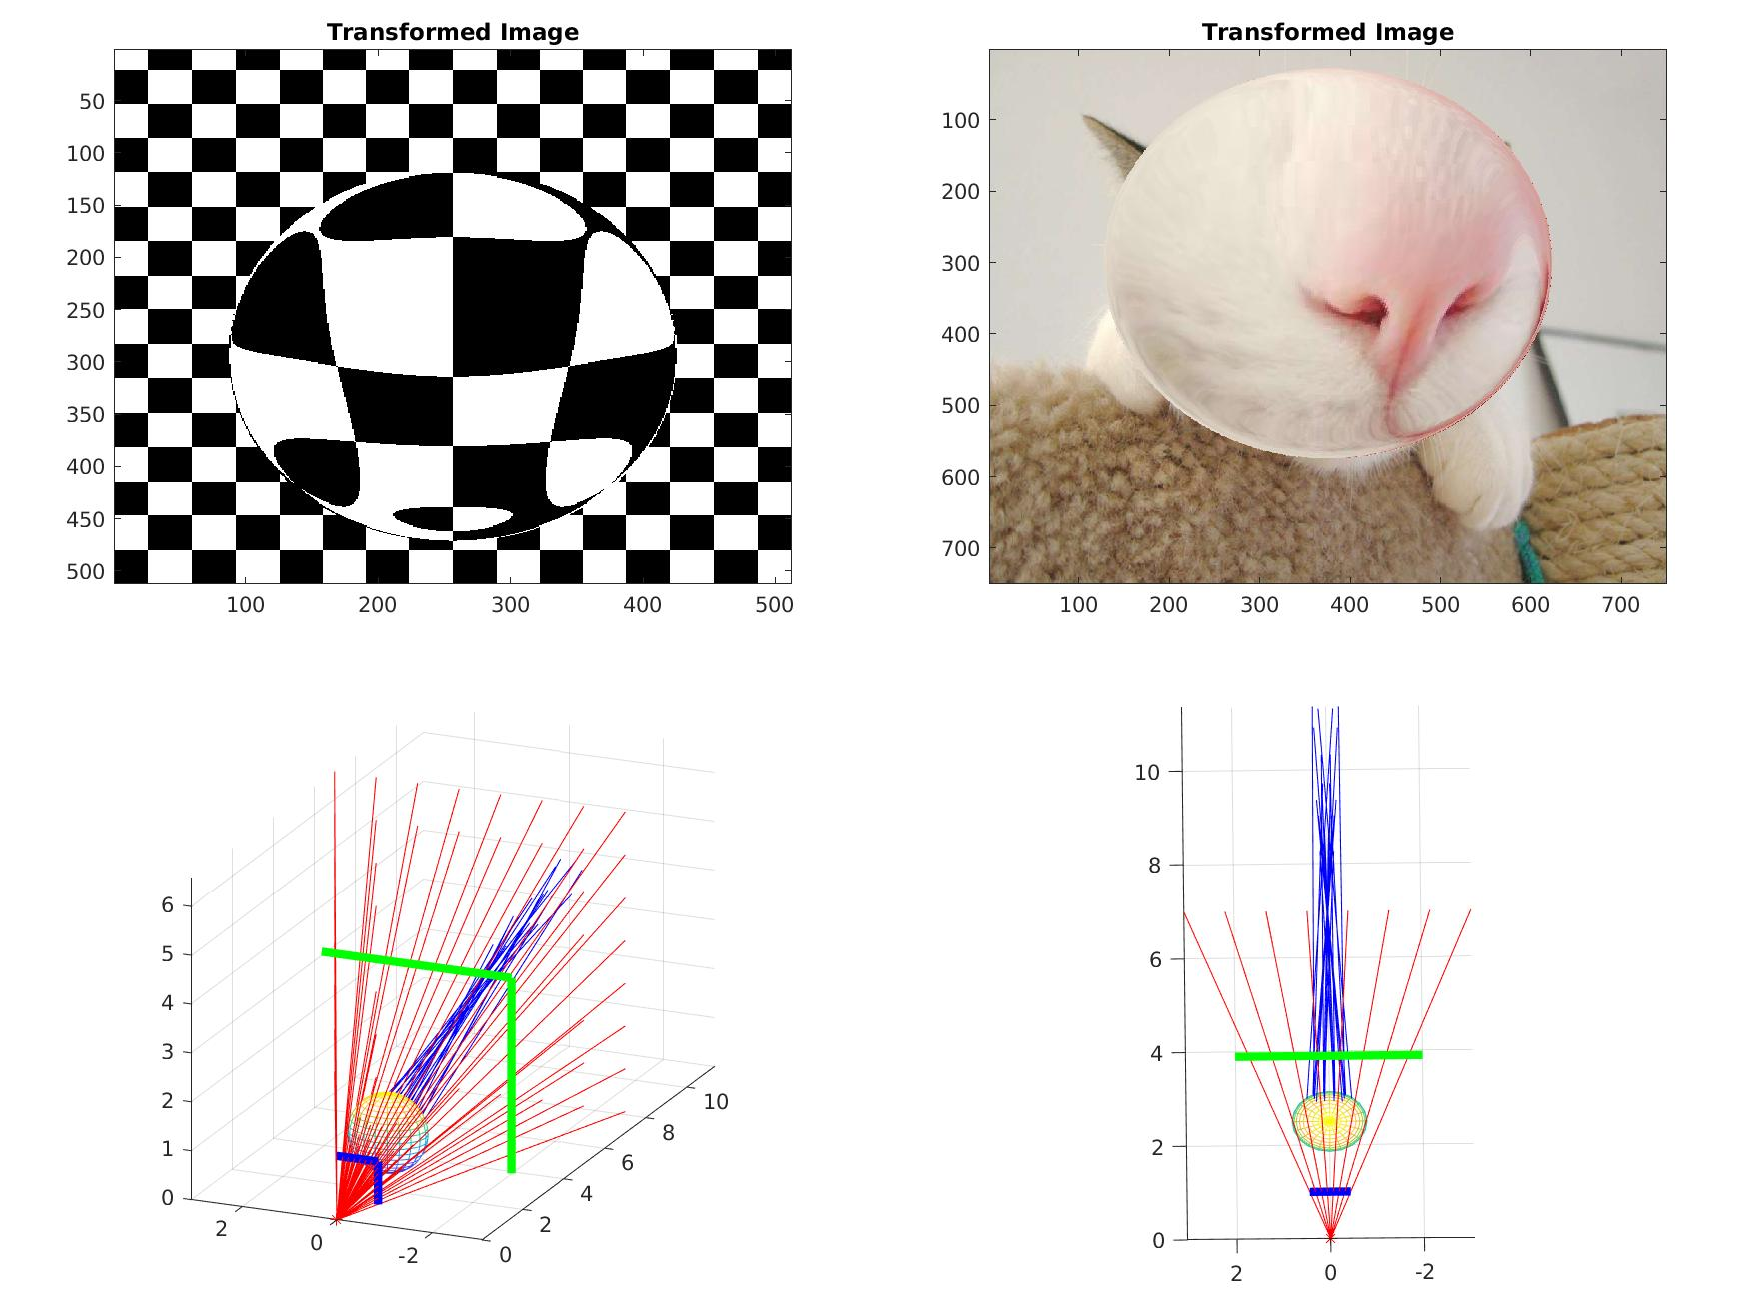
\includegraphics[scale=0.18]{2}
\captionof{figure}{Applying an Ellipsoidal lens with an 0.8 Scaling factor in the x Direction}

\vspace{10mm}

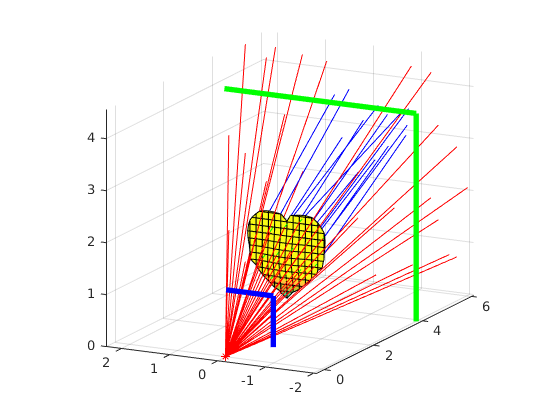
\includegraphics[scale=0.7]{4}
\captionof{figure}{Visualizing the Screens and The Taubin's Heart lens}

\vspace{10mm}


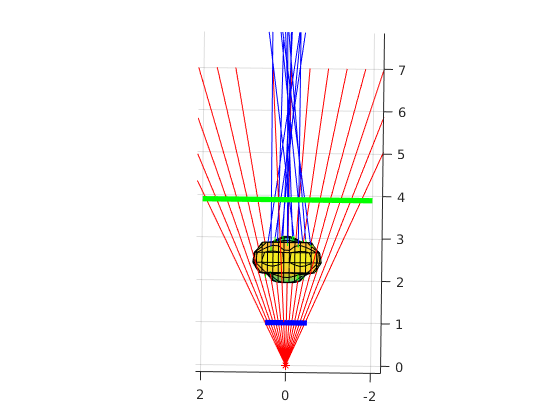
\includegraphics[scale=0.7]{5}
\captionof{figure}{Top Down View of the Screens and The Taubin's Heart lens}

\vspace{10mm}


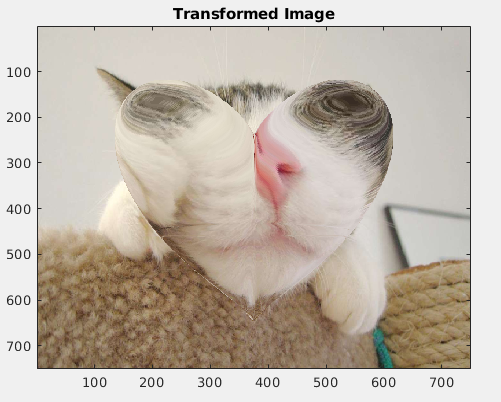
\includegraphics[scale=0.8]{6}
\captionof{figure}{The Cat Image transformed through a Taubin's heart scaled by a factor 0.2 in the x direction}

\vspace{10mm}

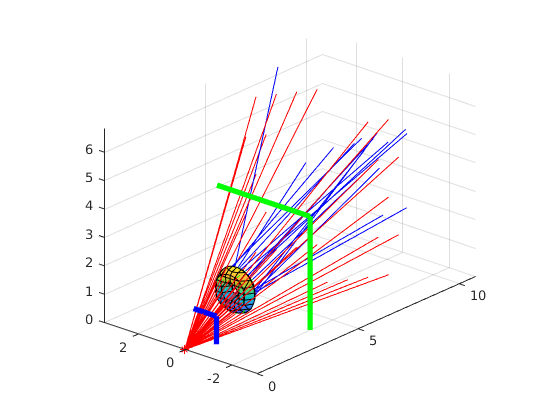
\includegraphics[scale=0.6]{7}
\captionof{figure}{Visualization of the light source, screens and lens configuration}

\vspace{10mm}

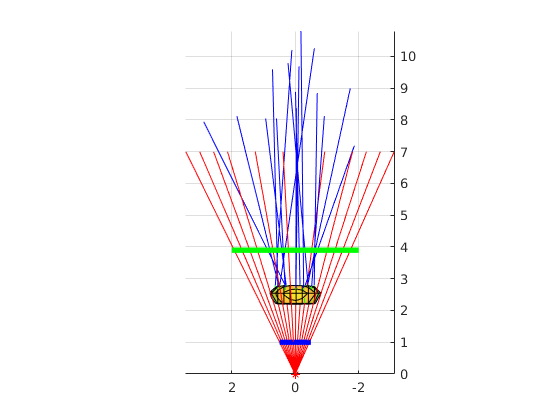
\includegraphics[scale=0.6]{8}
\captionof{figure}{Top Down View of the light source, screens and lens configuration}

\vspace{10mm}

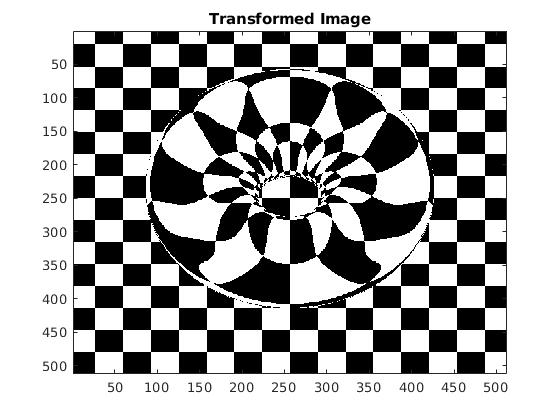
\includegraphics[scale=0.6]{9}
\captionof{figure}{Applying Torical lens to the Checkers pattern}

\vspace{10mm}

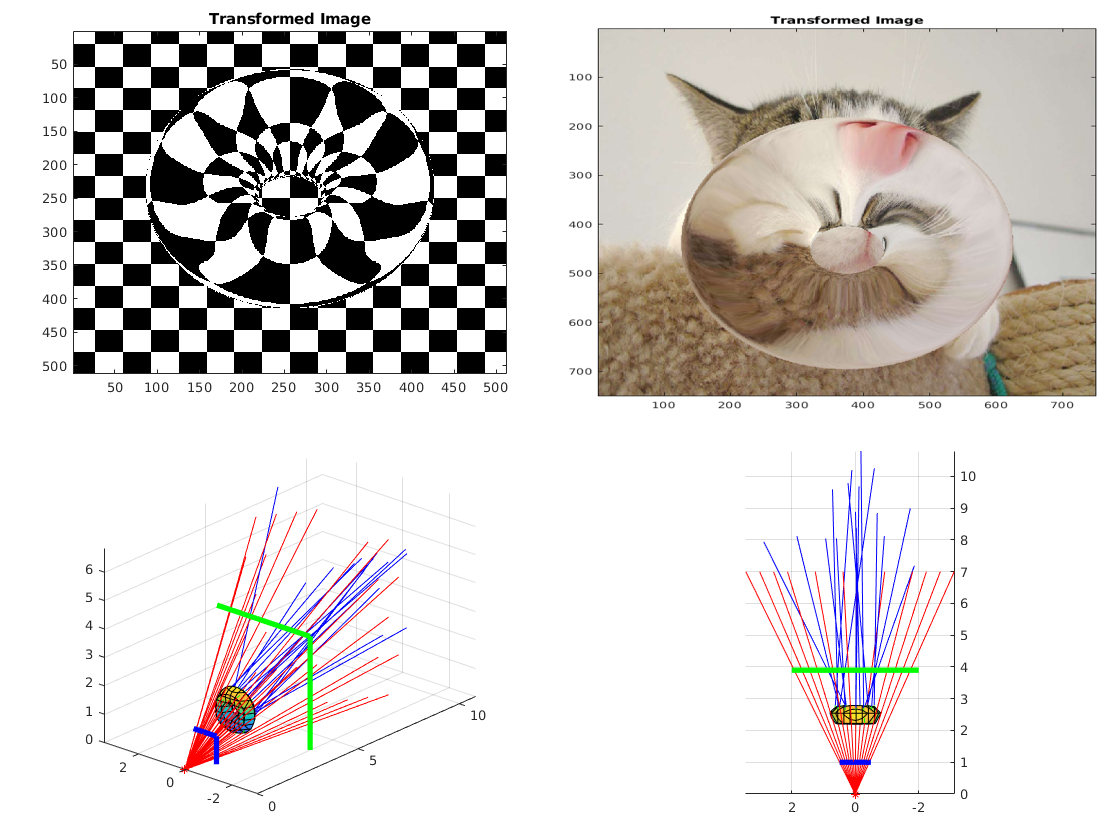
\includegraphics[scale=0.3]{10}
\captionof{figure}{Results of Applying torical lens}

\vspace{10mm}

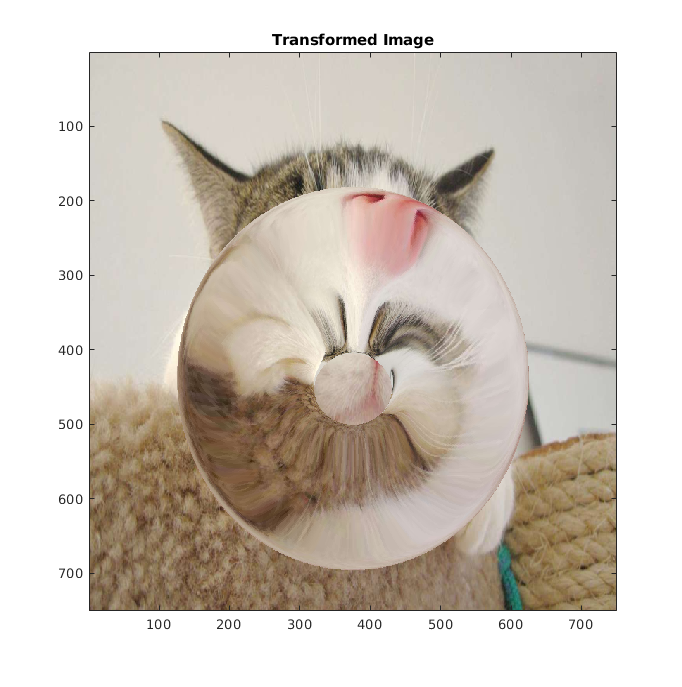
\includegraphics[scale=0.8]{11}
\captionof{figure}{Image of a Cat Lensed with a torical lens}

\vspace{10mm}

\newpage

\section{Sources}
\begin{itemize}
  \item https://en.wikipedia.org/wiki/Refraction
  \item https://en.wikipedia.org/wiki/Snell%27s_law
  \item http://www.starkeffects.com/snells-law-vector.shtml
  \item Zakrajsek Egon. Matematicno Modeliranje. DMFA \- zaloznistvo, 2004.
  \item Strang, Gilbert. Introduction to Linear Algebra. Wellesley-Cambridge Press, 2016.
\end{itemize}
\end{document}